\documentclass[seminarskirad]{fer}

\usepackage{blindtext}

%--- PODACI O RADU / THESIS INFORMATION ----------------------------------------

% Naslov na engleskom jeziku / Title in English
\title{Bamboo Filter}

% Naslov na hrvatskom jeziku / Title in Croatian
\naslov{Bamboo Filter}

% Autor / Author
\author{Petra Buršić i Nikola Kušen}

% Mentor 
\mentor{Prof.\@ Mirjana Domazet-Lošo}

% Datum rada na engleskom jeziku / Date in English
\date{May, 2024}

% Datum rada na hrvatskom jeziku / Date in Croatian
\datum{svibanj, 2024.}

%-------------------------------------------------------------------------------

\begin{document}
	
	% Naslovnica se automatski generira / Titlepage is automatically generated
	\maketitle
	
	
	%--- SAŽETAK / ABSTRACT --------------------------------------------------------
	
	% Sažetak na hrvatskom
	\begin{sazetak}
		Ovaj rad bavi se istraživanjem i implementacijom Bamboo filtera, napredne strukture podataka za upite približnog članstva (AMQ). Bamboo filter je osmišljen kako bi riješio probleme koji su prisutni u drugim AMQ strukturama kao što su Bloom filteri, cuckoo filteri i XOR filteri. Glavni ciljevi Bamboo filtera su omogućiti neblokirajuće povećanje kapaciteta i smanjiti degradaciju performansi prilikom povećanja strukture. U našoj implementaciji, nastojali smo replicirati funkcionalnosti originalnog Bamboo filtera te usporediti performanse naše implementacije s originalnom. Kroz analizu rezultata, prikazali smo prednosti i nedostatke naše implementacije.
	\end{sazetak}
	
	\begin{kljucnerijeci}
		Bamboo filter; Cuckoo filter; AMQ
	\end{kljucnerijeci}
	
	% Sadržaj se automatski generira / Table of contents is automatically generated
	\tableofcontents
	
	%--- UVOD / INTRODUCTION -------------------------------------------------------
	\chapter{Uvod}
	\label{pog:uvod}
	
	Ovaj rad pisan je kao projekt na predmetu Bioinformatika 1 gdje nam je zadatak bio istražiti i implementirati Bamboo filter. To je struktura podataka za upite približnog članstva (eng. Approximate membership query data structure ili AMQ). Ime dolazi od načina korištenja tih struktura podataka kojima postavljamo upite tipa "Je li X član ove strukture", a kao odgovor dobijemo ili da je X \textit{možda} u strukturi ili da \textit{sigurno} nije. Drugim riječima, AMQ strukture mogu dati lažno pozitivan rezultat, ali ne i lažno negativan.
	
	Neke AMQ strukture podataka osim bamboo filtera su bloom filteri, cuckoo filteri i XOR filteri, a osnovna motivacija iza bamboo filtera je rješavanje dva problema koji postoje kod ostalih AMQ struktura. Svaka struktura ponekad se treba povećati kako bi se napravilo mjesta za nove podatke. Prvi problem koji se tu javlja jest da je povećanje strukture blokirajuća operacija, to jest ne možemo raditi ništa drugo sa strukturom kada je ona u procesu povećanja. Drugi problem je degradacija performansi, odnosno povećanje vremena potrebnog za odgovoriti na upit u odnosu na ono prije povećanja strukture.
	
	
	%-------------------------------------------------------------------------------
	\chapter{Glavni dio}
	\label{pog:glavni_dio}
	
	\section{Struktura Bamboo Filtera}
	Bamboo filter se sastoji od četiri sloja podataka: hash tablice, segmenta, kantice (bucket) i ulaza (entry). Ulaz je osnovna jedinica Bamboo filtera, gdje se svaki element pohranjuje kao otisak (fingerprint) u ulazu. Više ulaza čini kanticu, koja je osnovna jedinica hash mapiranja tijekom umetanja, pretraživanja i brisanja. Segment je uveden između hash tablice i kantice, a niz uzastopnih kantica formira segment, dok niz segmenata čini hash tablicu. Svaki segment je zapravo jednostavni cuckoo filter. \cite{wang2022bamboo}.
	
	\section{Cuckoo Filter}
	Cuckoo filter je napredna struktura podataka za upite približnog članstva koja koristi princip premještanja (cuckooing) za postizanje visoke učinkovitosti i niskog postotka lažnih pozitivnih rezultata. Cuckoo filteri koriste dvije ili više hash funkcija za mapiranje svakog elementa na dvije ili više potencijalnih mjesta u tablici. Ako su sva potencijalna mjesta zauzeta, jedan od već pohranjenih elemenata se premješta na alternativno mjesto, oslobađajući prostor za novi element \cite{fan2013cuckoo}.
	
	Prednosti cuckoo filtera uključuju:
	\begin{itemize}
		\item Manji postotak lažno pozitivnih rezultata u usporedbi s Bloom filterima.
		\item Dinamično prilagođavanje veličine filtera bez potrebe za ponovnim hashiranjem svih elemenata \cite{fan2014cuckoo}.
	\end{itemize}
	
	Primjena cuckoo filtera u Bamboo filterima omogućuje efikasno i fleksibilno povećanje kapaciteta uz minimalnu degradaciju performansi.
	
	
	\section{Algoritmi Bamboo Filtera}
	Ovaj odjeljak opisuje glavne algoritme korištene u implementaciji Bamboo filtera, uključujući umetanje, proširenje, uklanjanje, pretragu i kompresiju \cite{wang2022bamboo}.
	
	\subsection{Algoritam Umetanja}
	Algoritam umetanja u Bamboo filter temelji se na izračunu otiska, primarne i alternativne kante te segmenta. Postupak uključuje izračunavanje otiska, provjeru slobodnih mjesta u primarnoj i alternativnoj kantici, te prebacivanje (cuckooing) ako su obje kantice pune.
	
	\subsection{Algoritam Proširenja}
	Algoritam proširenja osigurava dodavanje novih segmenata kako bi se omogućilo umetanje novih elemenata bez značajnog smanjenja performansi. Proširenje se pokreće kada se umetne određeni broj novih elemenata.
	
	\subsection{Algoritam Uklanjanja}
	Algoritam uklanjanja omogućava uklanjanje elemenata iz Bamboo filtera. Elementi se uklanjaju iz primarne ili alternativne kantice u segmentu, a ako je segment prepunjen, element se uklanja iz segmenta preljeva.
	
	\subsection{Algoritam Pretrage}
	Algoritam pretrage provjerava je li određeni element prisutan u Bamboo filteru. Elementi se traže u primarnoj i alternativnoj kantici u segmentu, a ako je segment prepunjen, traže se i u segmentu preljeva.
	
	\subsection{Algoritam Kompresije}
	Algoritam kompresije smanjuje veličinu Bamboo filtera uklanjanjem posljednjeg segmenta prebacivanjem njegovih elemenata.
	
	
	\section{Ilustracija Primjera Umetanja}
	\subsection{Početna Struktura}
	Na početku, Bamboo filter sastoji se od četiri segmenta, svaki segment ima četiri kantice. U svakom segmentu se nalaze otisci (fingerprints) kao što je prikazano na slici \ref{fig:initial_segments}.
	
	
	\begin{figure}[h]
		\centering
		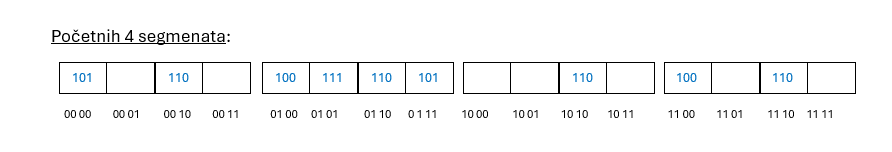
\includegraphics[width=0.9\textwidth]{images/initial_segments.png}
		\caption{Početna struktura Bamboo filtera sa četiri segmenta.}
		\label{fig:initial_segments}
	\end{figure}
	
	\subsection{Umetanje Elementa e1}
	Kada želimo umetnuti element \( e1 \) s hash vrijednosti \( \text{hash}(e1) = 1110000 \) u Bamboo filter, slijedeći koraci se događaju:
	\begin{itemize}
		\item Izračun otiska, segmentnog indeksa i indeksa kantice.
		\item Primarna kantica nije dostupna, otisak se premješta u alternativnu kanticu.
		\item Ako je ovo dodavanje okinulo proširenje, dodaje se novi, 5. segment te otisak 111 ide u njega jer se sad za indeks segmenta gleda i zadnji bit otiska (101 = 5)
	\end{itemize}
	Ilustracija ovog procesa prikazana je na slici \ref{fig:insertion_e1}.
	
	\begin{figure}[h]
		\centering
		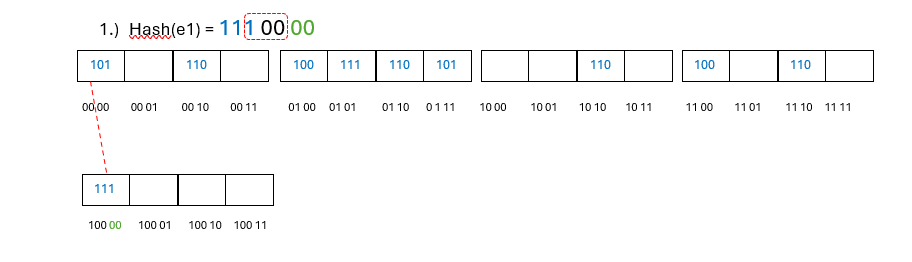
\includegraphics[width=0.9\textwidth]{images/umetanje_el1.png}
		\caption{Umetanje elementa \( e1 \) s hash vrijednosti \( 1110000 \).}
		\label{fig:insertion_e1}
	\end{figure}
	
	\subsection{Umetanje Elementa e2}
	Sljedeći primjer prikazuje umetanje elementa \( e2 \) s hash vrijednosti \( \text{hash}(e2) = 1010101 \) u Bamboo filter. Koraci umetanja:
	\begin{itemize}
		\item Izračun otiska, segmentnog indeksa i indeksa kantice.
		\item Primarna kantica nije dostupna, otisak se premješta u alternativnu kanticu.
		\item Ako je ovo dodavanje okinulo proširenje, dodaje se novi, 6. segment za smještaj novog otiska 101.
	\end{itemize}
	Ilustracija ovog procesa prikazana je na slici \ref{fig:insertion_e2}.
	
	\begin{figure}[h]
		\centering
		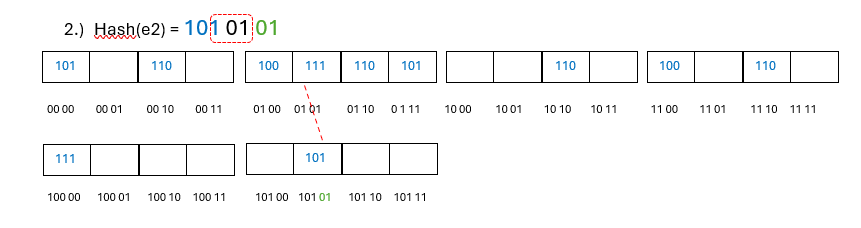
\includegraphics[width=0.9\textwidth]{images/umetanje_el2.png}
		\caption{Umetanje elementa \( e2 \) s hash vrijednosti \( 1010101 \).}
		\label{fig:insertion_e2}
	\end{figure}
	

%-------------------------------------------------------------------------------
\chapter{Rezultati i rasprava}
\label{pog:rezultati_i_rasprava}

\section{Testiranje na umjetno generiranim podatcima}
Testirali smo našu i originalnu implementaciju na 10 različitih uzoraka različite duljine u intervalu \(10^3\) - \(10^7\) znakova. \\


Naša implementacija na nasumičnim uzorcima s k=10:
\begin{center}
	\small
	\begin{tabular}{||c c c c c||} 
		\hline
		Duljina uzorka & Vrijeme izvođenja & Memorija & Preciznost & Lažno pozitivno \\ [0.5ex] 
		\hline\hline
		200 & 0.004s & 228.4KB & 100\% & 0\% \\ 
		\hline
		500 & 0.005s & 228.7KB & 100\% & 0\% \\
		\hline
		1000 & 0.005s & 229.1KB & 100\% & 0\% \\
		\hline
		5000 & 0.005s & 249.2KB & 100\% & 0\% \\
		\hline
		10000 & 0.006s & 270.2KB & 100\% & 0\% \\
		\hline
		50000 & 0.012s & 470.1KB & 100\% & 0\% \\ 
		\hline
		100000 & 0.022s & 718.7KB & 100\% & 0\% \\
		\hline
		500000 & 0.111s & 2.601MB & 100\% & 0\% \\
		\hline
		1000000 & 0.23s & 6.426MB & 100\% & 0\% \\
		\hline
		5000000 & 1.847s & 58.81MB & 100\% & 0\% \\ [1ex] 
		\hline
	\end{tabular}
\end{center}

Originalna implementacija na nasumičnim uzorcima s k=10:

\begin{center}
	\small
	\begin{tabular}{||c c c c c||} 
		\hline
		Duljina uzorka & Vrijeme izvođenja & Memorija & Preciznost & Lažno pozitivno \\ [0.5ex] 
		\hline\hline
		200 & 0.004s & 197.9KB & 100\% & 0\% \\ 
		\hline
		500 & 0.004s & 198.2KB & 100\% & 0\% \\
		\hline
		1000 & 0.004s & 198.7KB & 100\% & 0\% \\
		\hline
		5000 & 0.004s & 202.6KB & 100\% & 0\% \\
		\hline
		10000 & 0.004s & 213.7KB & 100\% & 0\% \\
		\hline
		50000 & 0.007s & 349.4KB & 100\% & 0\% \\ 
		\hline
		100000 & 0.011s & 573.1KB & 100\% & 0\% \\
		\hline
		500000 & 0.64s & 2.17MB & 100\% & 0\% \\
		\hline
		1000000 & 0.128s & 4.55MB & 99.5\% & 1\% \\
		\hline
		5000000 & 0.634s & 27.05MB & 97.5\% & 4.76\% \\ [1ex] 
		\hline
	\end{tabular}
\end{center}


U nastavku su prikazani grafovi koji uspoređuju vrijeme izvođenja, iskorištenu memoriju, preciznost i postotak lažno pozitivnih rezultata za obje implementacije.

\section{Vrijeme izvođenja}
\begin{figure}[h]
	\centering
	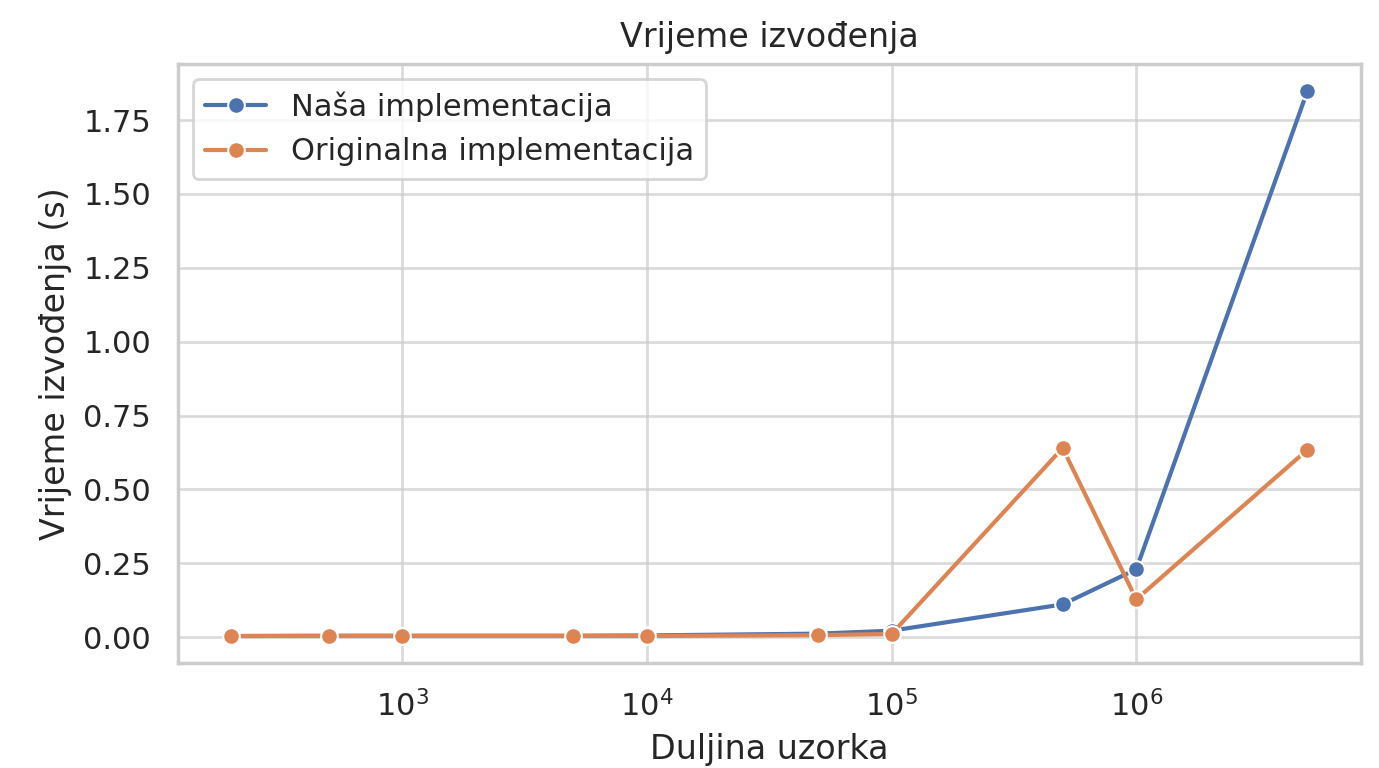
\includegraphics[width=0.9\textwidth]{images/nasumicni_rezultati_vrijeme.png}
	\label{fig:nasumicni_rezultati_vrijeme}
\end{figure}
Na grafu, prva slika prikazuje vrijeme izvođenja za različite duljine uzoraka. Naša implementacija pokazuje konzistentno vrijeme izvođenja za manje uzorke, ali vrijeme značajno raste za veće uzorke. Originalna implementacija ima stabilnije vrijeme izvođenja za veće uzorke.

\section{Iskorištena memorija}
\begin{figure}[h]
	\centering
	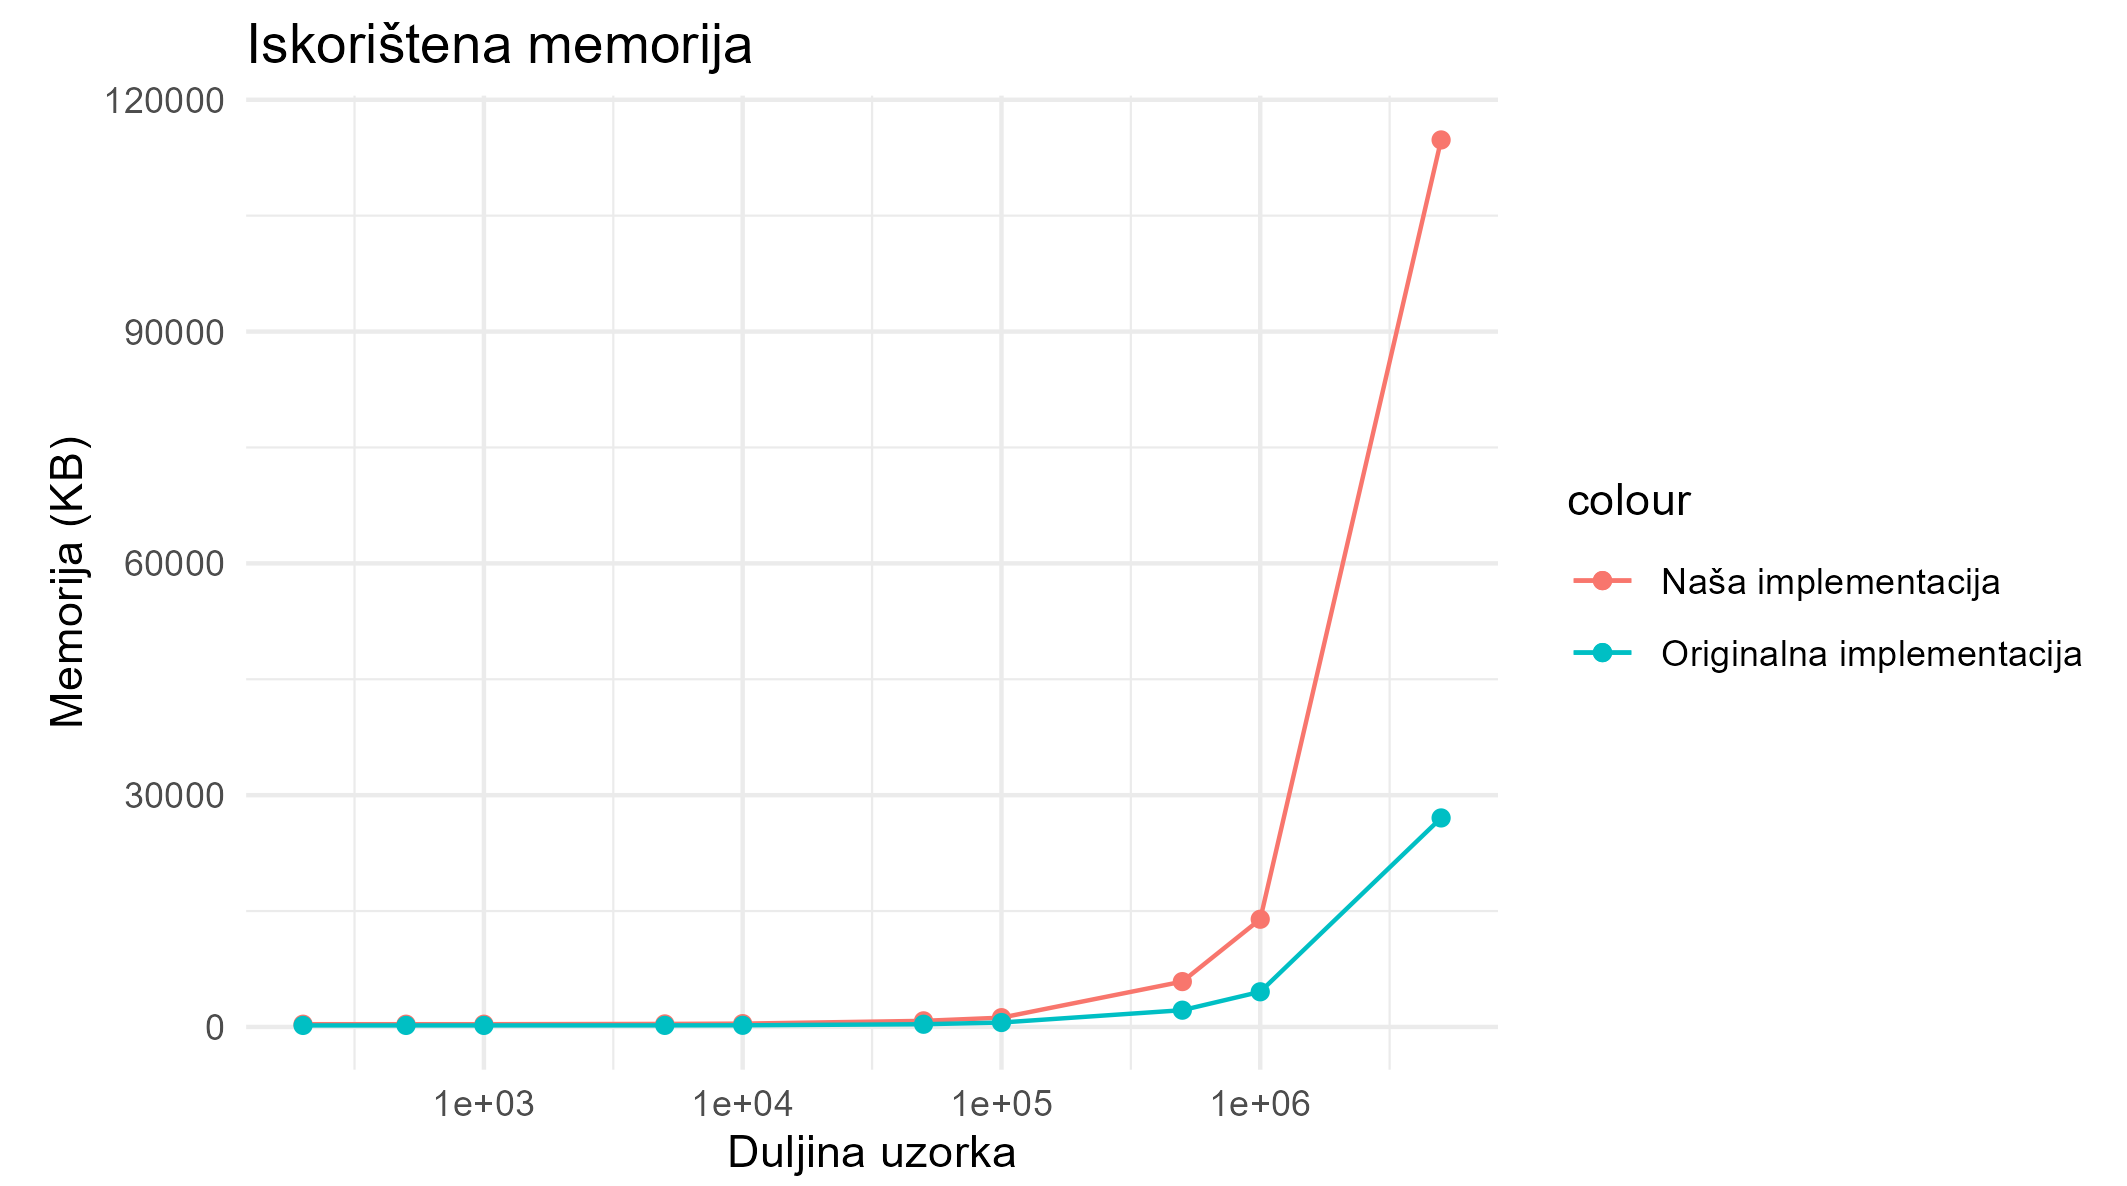
\includegraphics[width=0.9\textwidth]{images/nasumicni_rezultati_memorija.png}
	\label{fig:nasumicni_rezultati_memorija}
\end{figure}
Druga slika prikazuje iskorištenu memoriju za različite duljine uzoraka. Naša implementacija koristi više memorije, pogotovo za veće uzorke, dok originalna implementacija pokazuje umjereno povećanje memorije za veće uzorke.

\section{Preciznost}
\begin{figure}[h]
	\centering
	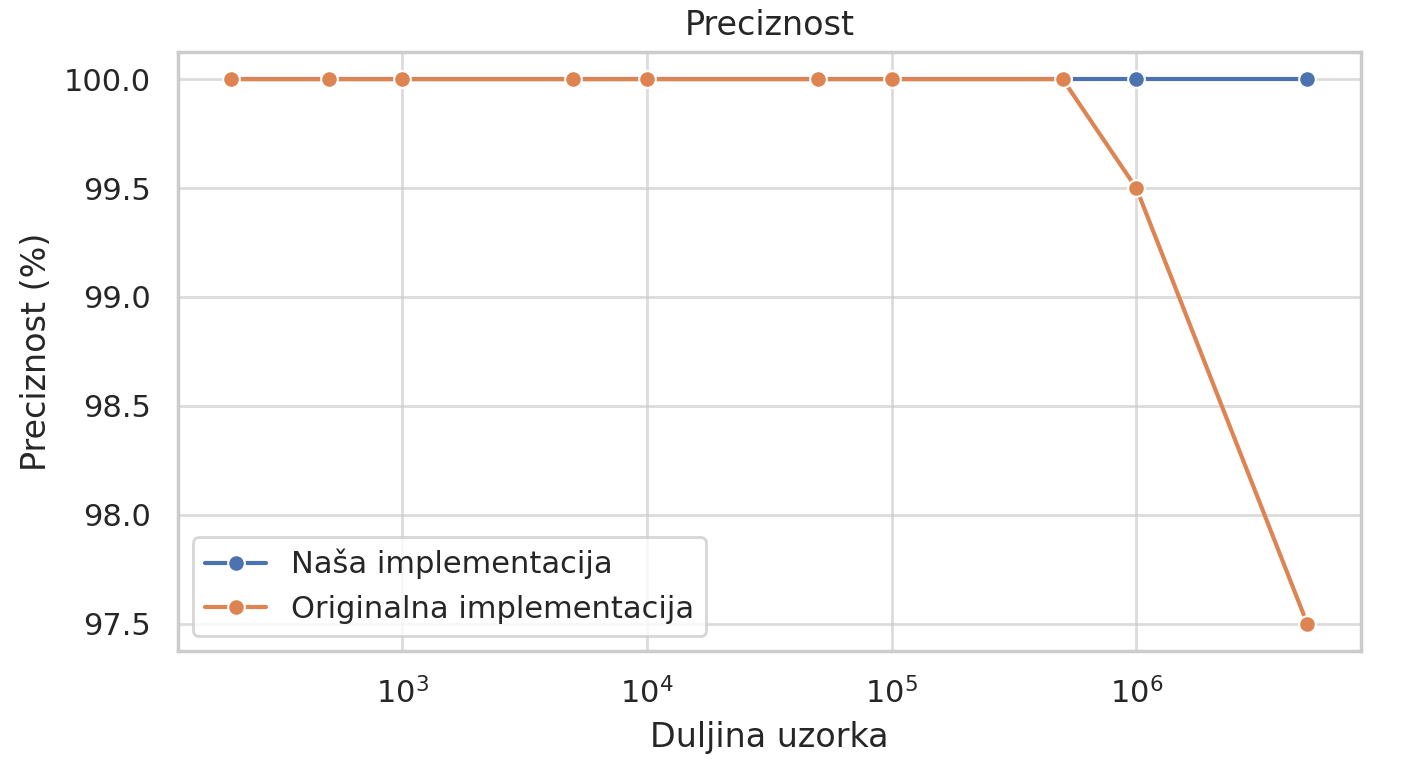
\includegraphics[width=0.9\textwidth]{images/nasumicni_rezultati_preciznost.png}
	\label{fig:nasumicni_rezultati_preciznost}
\end{figure}
Treća slika prikazuje preciznost obiju implementacija. Naša implementacija održava maksimalnu preciznost za sve uzorke, dok originalna implementacija ima blagi pad preciznosti za najveće uzorke.

\section{Lažno pozitivno}
\begin{figure}[h]
	\centering
	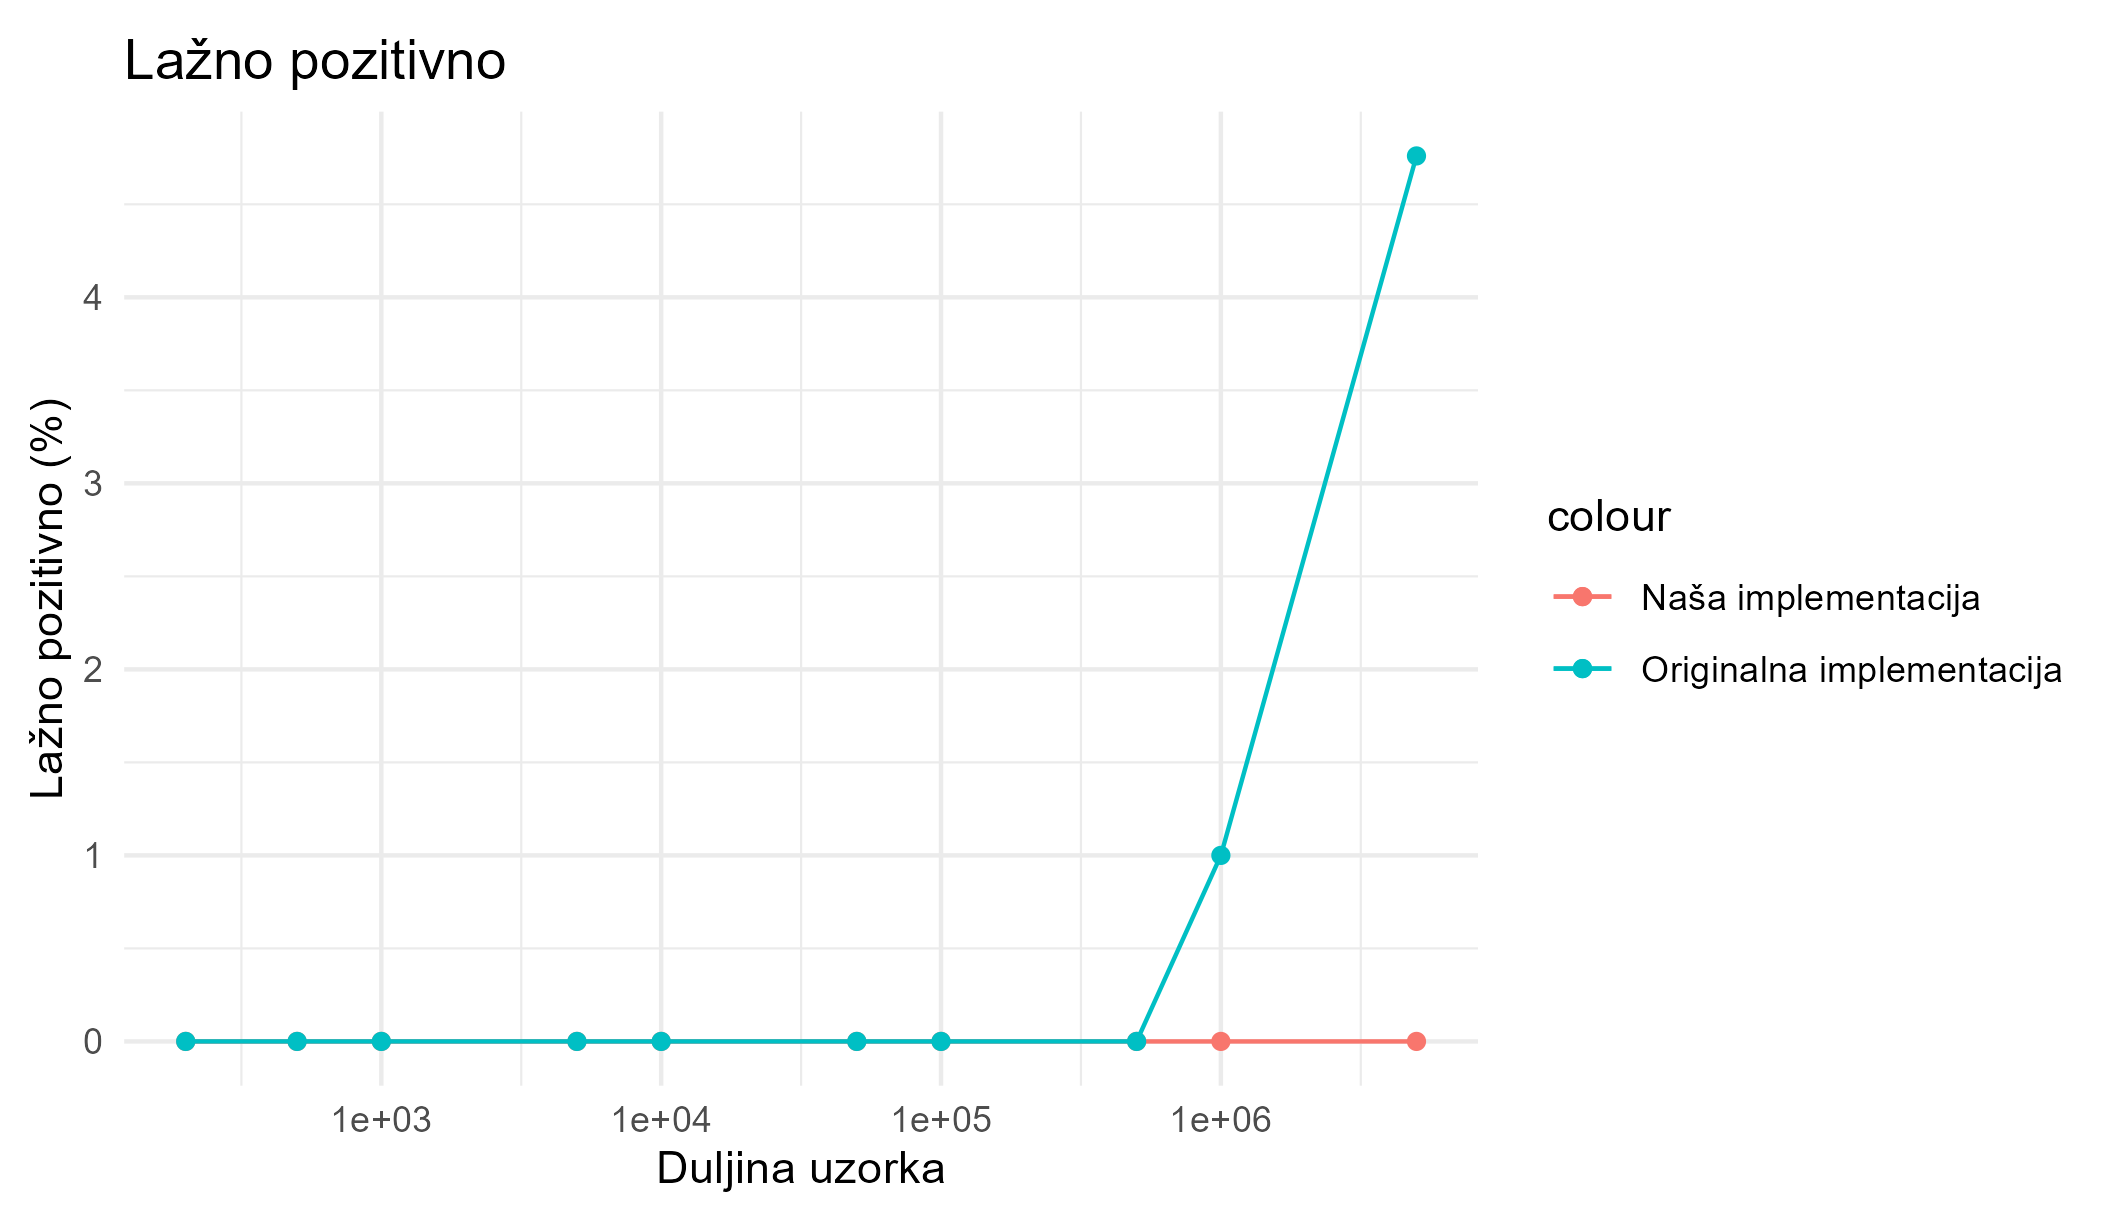
\includegraphics[width=0.9\textwidth]{images/nasumicni_rezultati_lazno.png}
	\label{fig:nasumicni_rezultati_lazno}
\end{figure}
Četvrta slika prikazuje postotak lažno pozitivnih rezultata. Naša implementacija ne pokazuje lažno pozitivne rezultate, dok originalna implementacija pokazuje povećanje lažno pozitivnih rezultata za veće uzorke.

Ovi rezultati pokazuju da naša implementacija pruža veću preciznost bez lažno pozitivnih rezultata, ali dolazi s cijenom većeg vremena izvođenja i veće memorijske potrošnje za veće uzorke u usporedbi s originalnom implementacijom.


\section{Testiranje na stvarnim podatcima (Escherichia coli)}
Naša implementacija na genomu \textit{E. coli} (4641652 baza) s različitim k:

\begin{center}
	\small
	\begin{tabular}{||c c c c c||} 
		\hline
		k & Vrijeme izvođenja & Memorija & Preciznost & Lažno pozitivno \\ [0.5ex] 
		\hline\hline
		10 & 2.495s & 104.7MB & 99.5\% & 1\% \\ 
		\hline
		20 & 1.21s & 32.44MB & 100\% & 0\% \\
		\hline
		50 & 1.203s & 28.74MB & 99.5\% & 1\% \\
		\hline
		100 & 1.234s & 27.91MB & 99\% & 1.96\% \\
		\hline
		200 & 1.28s & 27.01MB & 100\% & 0\% \\ [1ex] 
		\hline
	\end{tabular}
\end{center}

Originalna implementacija na genomu \textit{E. coli} (4641652 baza) s različitim k:

\begin{center}
	\small
	\begin{tabular}{||c c c c c||} 
		\hline
		k & Vrijeme izvođenja & Memorija & Preciznost & Lažno pozitivno \\ [0.5ex] 
		\hline\hline
		10 & 0.621s & 39.83MB & 99\% & 1.96\% \\ 
		\hline
		20 & 0.659s & 22.23MB & 92\% & 13.79\% \\
		\hline
		50 & 0.774s & 21.84MB & 92\% & 13.79\% \\
		\hline
		100 & 0.877s & 21.8MB & 93\% & 12.28\% \\
		\hline
		200 & 1.192s & 21.8MB & 96\% & 8.26\% \\ [1ex] 
		\hline
	\end{tabular}
\end{center}

U nastavku su prikazani grafovi koji uspoređuju vrijeme izvođenja, iskorištenu memoriju, preciznost i postotak lažno pozitivnih rezultata za obje implementacije.

\begin{figure}[h]
	\centering
	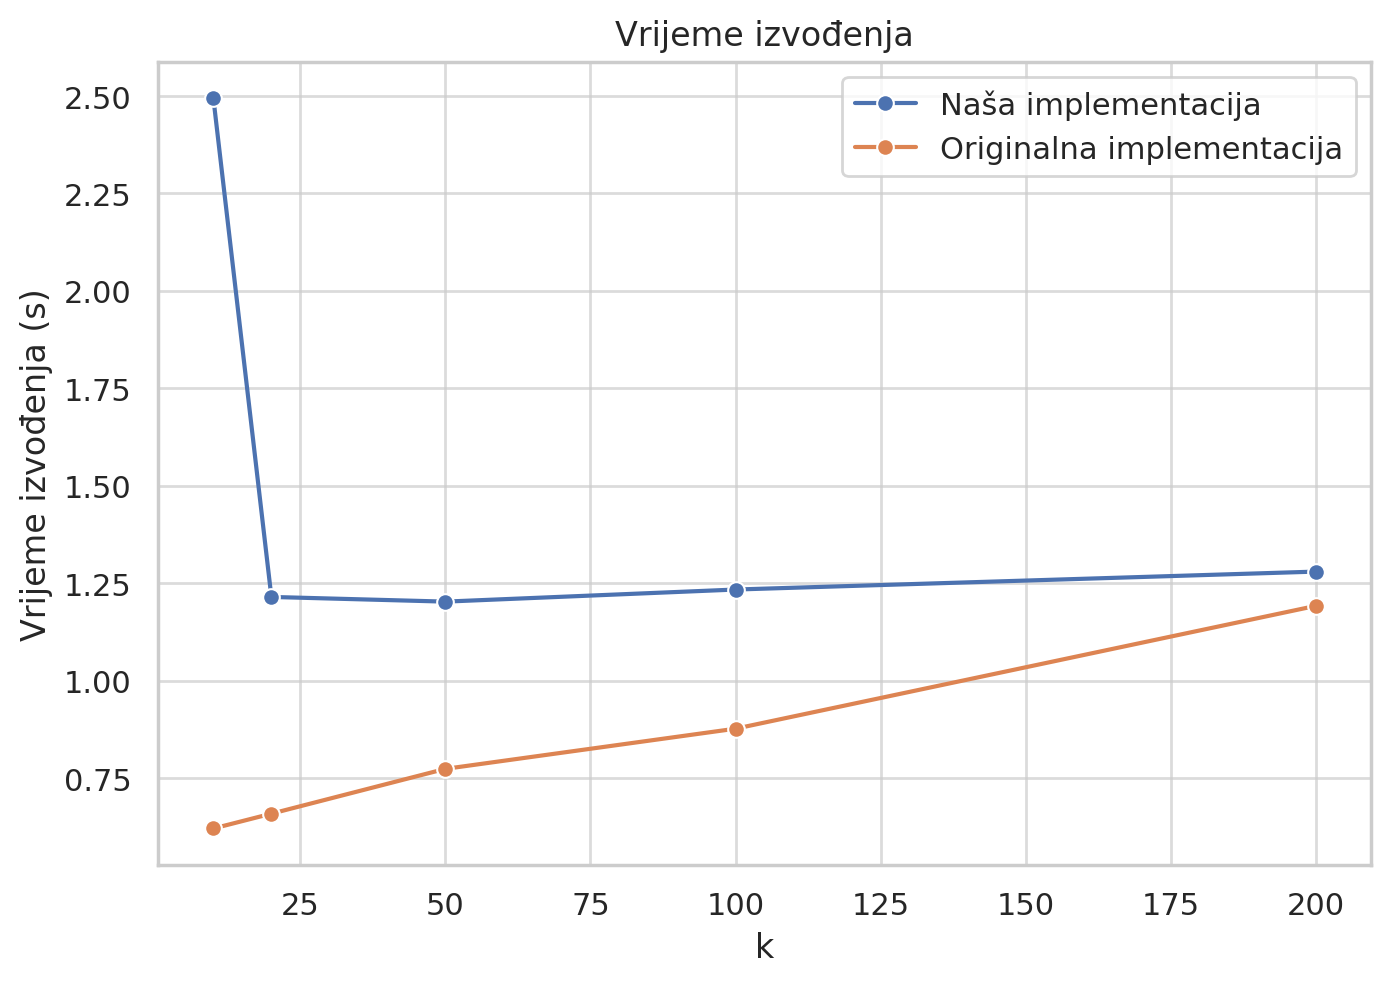
\includegraphics[width=0.9\textwidth]{images/EColi_rezultati_vrijeme.png}
	\caption{Graf vremena E. Coli.}
	\label{fig:EColi_rezultati_vrijeme}
\end{figure}
\begin{figure}[h]
	\centering
	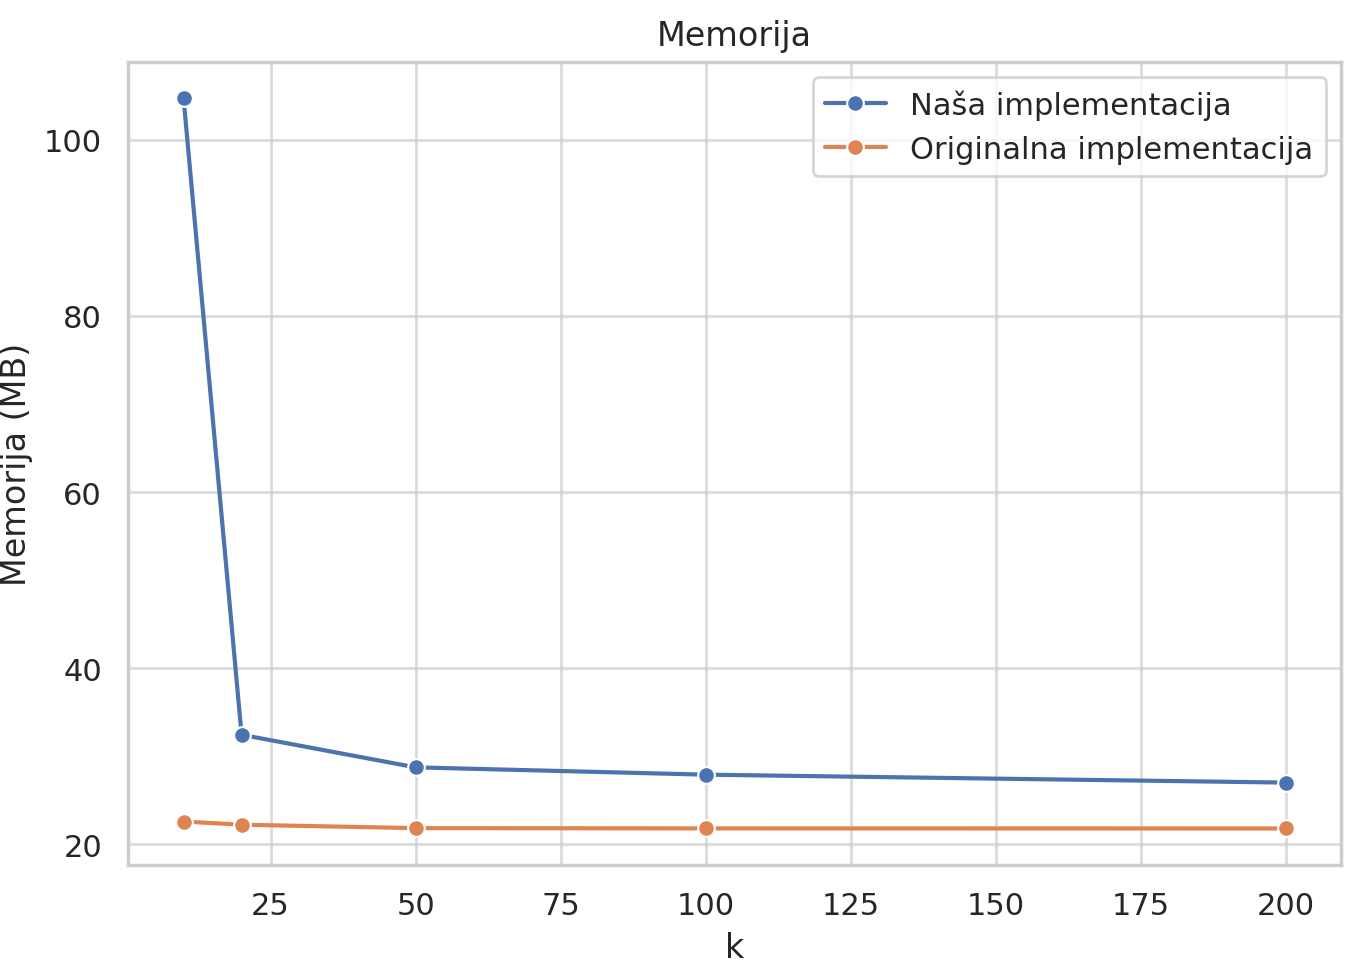
\includegraphics[width=0.9\textwidth]{images/EColi_rezultati_memorija.png}
	\caption{Graf memorije E. Coli.}
	\label{fig:EColi_rezultati_memorija}
\end{figure}
\begin{figure}[h]
	\centering
	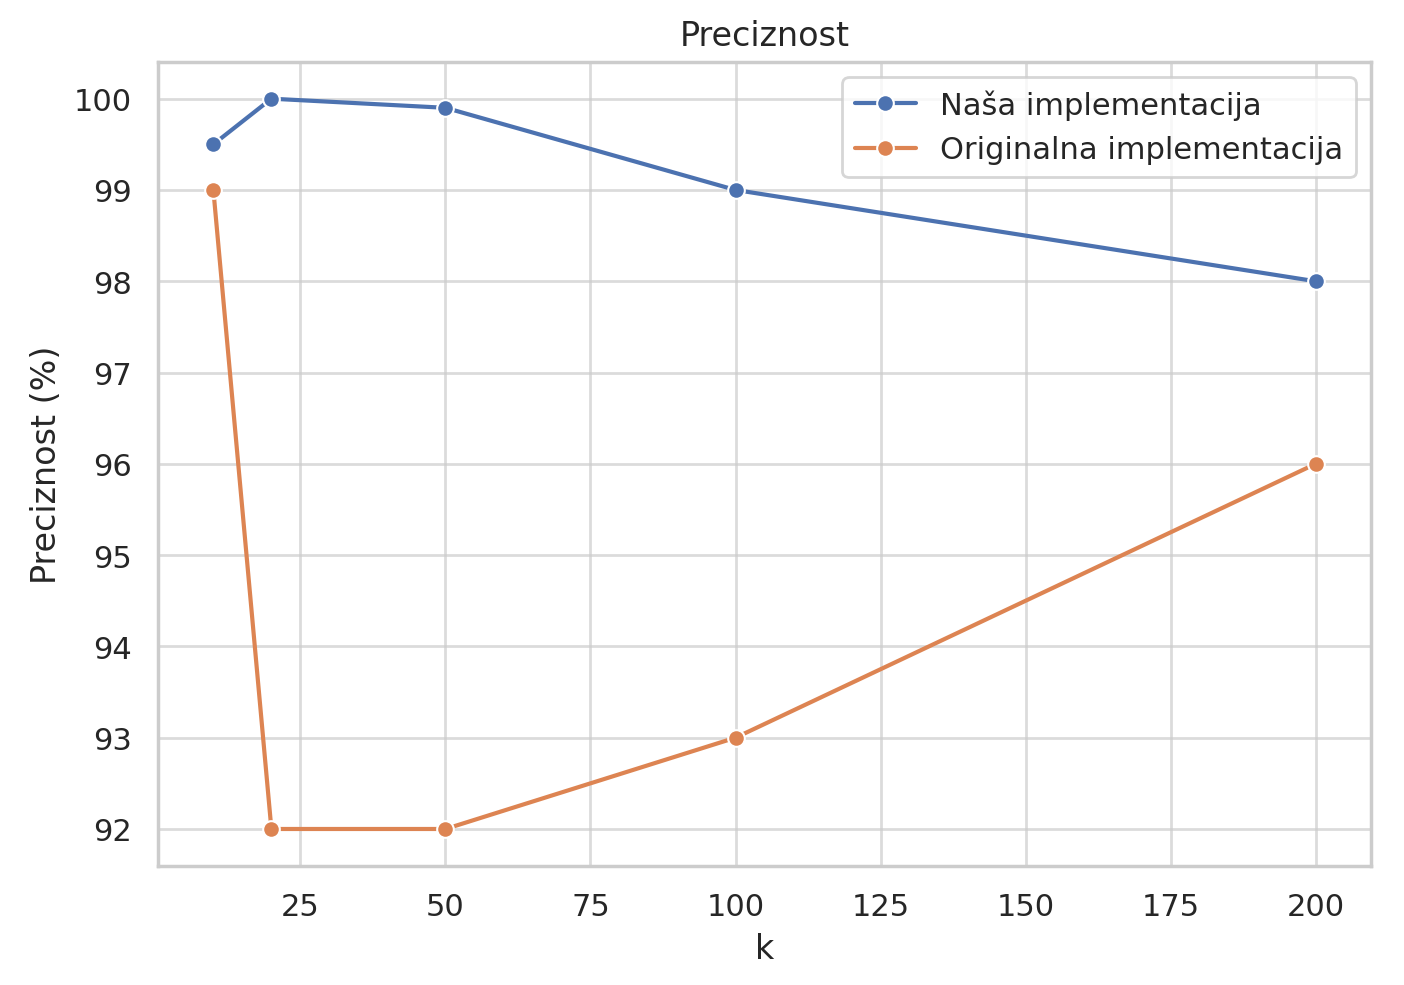
\includegraphics[width=0.9\textwidth]{images/EColi_rezultati_preciznost.png}
	\caption{Graf preciznosti E. Coli.}
	\label{fig:EColi_rezultati_preciznost}
\end{figure}
\begin{figure}[h]
	\centering
	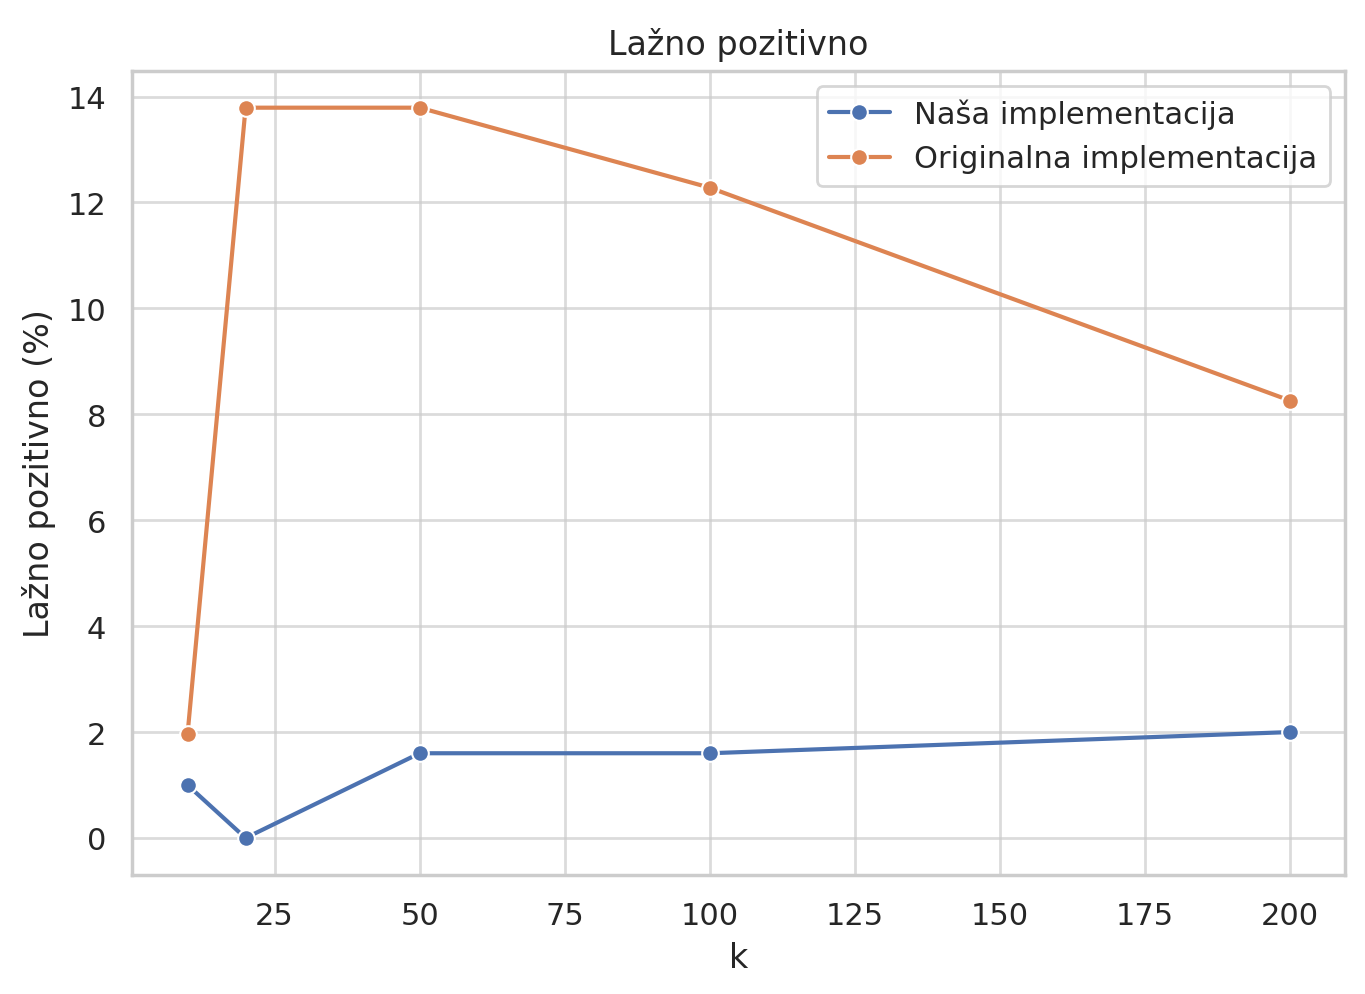
\includegraphics[width=0.9\textwidth]{images/EColi_rezultati_lazno.png}
	\caption{Graf lazno pozitivnih E. Coli.}
	\label{fig:EColi_rezultati_lazno}
\end{figure}


%--- ZAKLJUČAK / CONCLUSION ----------------------------------------------------
\chapter{Zaključak}
\label{pog:zakljucak}
U ovom radu predstavili smo Bamboo filter, naprednu strukturu podataka za upite približnog članstva (AMQ), te analizirali njegovu implementaciju i performanse. Naš cilj je bio replicirati funkcionalnosti originalnog Bamboo filtera te usporediti performanse naše implementacije s originalnom.

Naša implementacija pokazala je visoku preciznost, bez lažno pozitivnih rezultata na nasumičnim uzorcima i uzorcima iz genoma Escherichia coli. Međutim, visoka preciznost postignuta je uz cijenu većeg vremena izvođenja i veće memorijske potrošnje u usporedbi s originalnom implementacijom. Dok originalna implementacija pokazuje stabilniju memorijsku potrošnju i vrijeme izvođenja za veće uzorke, naša implementacija osigurava veću točnost.

Bamboo filter se sastoji od hash tablice u kojoj su spremljeni segmenti, gdje je svaki segment zapravo cuckoo filter. Ovo omogućava efikasno i fleksibilno povećanje kapaciteta uz minimalnu degradaciju performansi. Implementirani algoritmi za umetanje, proširenje, uklanjanje, pretragu i kompresiju omogućavaju robustno upravljanje i optimizaciju memorije.

Kroz analizu rezultata, prikazali smo prednosti i nedostatke naše implementacije, te identificirali područja za poboljšanja. 

Naša analiza pokazuje da Bamboo filter nudi značajne prednosti u pogledu preciznosti i fleksibilnosti u upravljanju kapacitetom, te predstavlja vrijednu alternativu postojećim AMQ strukturama kao što su Bloom filteri i cuckoo filteri.


%--- LITERATURA / REFERENCES ---------------------------------------------------

% Literatura se automatski generira / References are automatically generated
% Upiši ime BibTeX datoteke bez .bib nastavka / Enter the name of the BibTeX file without .bib extension
\bibliography{literatura}
\bibliographystyle{plain}


\end{document}
